\documentclass[
    a4paper,
    brazil
    ]{article}
    
\usepackage{cmap}
\usepackage[utf8]{inputenc}
\usepackage{graphicx}
\usepackage{subcaption}
\usepackage{fullpage}
\usepackage{mathtools}
\usepackage{wrapfig}
\usepackage{indentfirst}
\usepackage{verbatim}
\usepackage{float}
\usepackage{gensymb}
\usepackage[T1]{fontenc}
\usepackage[portuguese]{babel}
\usepackage[num]{abntex2cite}
\usepackage{booktabs,array,lmodern}

\begin{document}
% capa
\begin{titlepage} %iniciando a "capa"
\begin{center} %centralizar o texto abaixo
{\large Universidade de São Paulo}\\[0.2cm] %0,2cm � a dist�ncia entre o texto dessa linha e o texto da pr�xima
{\large EESC}\\[0.2cm] % o comando \\ "manda" o texto ir para pr�xima linha
{\large Departamento de Engenharia Elétrica}\\[0.2cm]
{\large Engenharia Elétrica - ênfase em Eletrôica}\\[2.5cm]
{\huge Aplicação de Microprocessadores II}\\[3.1cm]
\begin{figure}[h]
    
\includegraphics[scale=3]
    {imagens/usp.jpg}
    \centering
\end{figure}
{\bf \huge Prática 1}\\ % o comando \bf deixa o texto entre chaves em negrito. O comando \huge deixa o texto enorme
\end{center} %t�rmino do comando centralizar
{\centering
\large Paulo Augusto Alves Luz Viana    nºUSP 9313624\\Anderson Hiroshi Siqueira    nºUSP 9313197\\}%[0.7cm] % o comando \large deixa o texto grande

\begin{center}
{\large São Carlos}\\[0.2cm]
{\large 2017}
\end{center}
\end{titlepage} %t�rmino da "capa"

\newpage
\newpage

\tableofcontents
\newpage
\listoffigures
\newpage
%%\listoftables
%%\newpage


%   \begin{figure}[H]
%        \includegraphics[scale=0.6]
%        {terceiraordem.jpg}
%        \centering
%        \caption{Diagrama de Blocos do sistema de Fase M�nima}
%        \label{terceiraordem}
%    \end{figure}
 


\section{Introdução}

    Nesta prática foram realizadas várias implementações em Assembly e em C, no microcontrolador AT89S52, baseado em 8051. Todas as implementações em Assembly foram feitas também em C, com o objetivo de se compreender e entender o funcionamento da linguagem e do hardware.\\
    
    A programação em Assembly tende a ser mais complicada pela linguagem ser de muito baixo nível, mesmo em comparação a linguagem C. Porém, ela permite uma liberdade maior de acesso a memória e as portas do microcontrolador, de tal forma que também é necessário cuidado para não se invadir outras regiões do código. Em C, por outro lado, a programação se torna mais intuitiva, e visualmente mais organizada, permitindo ainda a utilização de bibliotecas. Portanto em Assembly pode-se obter uma eficiência extremamente alta em termos de memória e velocidade, porém o esforço depreendido será maior e dependendo do tamanho do seu código seja melhor usar a linguagem C, pois a diferença de perfomance não será tão grande.\\
    
    O protocolo de comunicação serial RS232 funciona enviando-se uma sequência de bits junto com os dados, de forma serial. Há o bit de ínicio (start bit), o stop bit (que pode ser mais de 1) que indica o fim da mensagem,  e o bit de paridade que pode ou não estar presente para garantir que a mensagem foi entregue corretamente. Para que a comunicação seja feita da forma correta, é necessário que quem recebe os bits os leia na mesma velocidade que quem enviou, ou com o mesmo \emph{baud rate}. O \emph{baud rate} mais comum e utilizado em todas as implementações desta prática foi de 9600 bits por segundo.\\
    
    
    Um display LCD é um painel que pode exibir caracteres ou números, tendo 1, 2 ou mais linhas de caracteres. Funciona por meio de um microcontrolador interno que pode ser configurado externamente através de seus pinos de dados (D0 à D7) e configurações (ENAB, R/W e R/S). Com as devidas combinações de valores lógicos nestes pinos pode-se escrever em sua tela, faze-la acender, mover o cursor de escrita
    e ler o que está gravado nele, por exemplo.\\
    
    O display de 7 segmentos é na realidade um conjunto de 7 leds ( ou 8, com o ponto decimal), dispostos de forma a representar um número, e até algumas letras, normalmente utilizado para ser uma saída visual de algum dado do sistema, ou algum indicador.\\
    
    
    
    

\section{Materiais e métodos} 
    \begin{description}
        \item[Kit CPU-8051-USB] Placa com o microcontrolador AT89S52, da ATMEL, baseado em 8051.
        \item[Módulo PRL-LCD-1602(LCD 16x2 Black light)] Painel LCD com o controlador HD44780.
        \item[Módulo PR-LED-BT( 8 leds e 10 botões)] Placa com pinos de entrada para escrita nos leds e saáda para leitura dos botões.   
        \item[Módulo PR -7SEG-4 (Display 7 segmentos de 4 dígitos  multiplexado)] Placa com 4 Displays de 7 segmentos de anodo comum, multiplexados por transistores ligados aos catodos dos leds.
        \item[4 Flat cables para conexão entre CPU e módulos] Cabos de conexão entre as placas e o microcontrolador.  
        \item[Cabo de programação USB] Cabo para conexão com o PC, para programar o AT89S52.
        \item[Cabo de comunicação RS232] Cabo de comunicação com o PC.
    \end{description}
    
    \subsection{Parte 1 - Comunicação Serial}
        Nesta parte foi implementada um comunicação serial entre o microcontrolador e o computador, com mensagens sendo enviadas de um para o outro. Foi utilizado os paretros (9600, 8, N, 1), que significa 9660 de \emph{baud rate}, com 8 bits de dados, sem bit de paridade e 1 stop bit. No PC os dados foram recebidos através do teclado pelo terminal do software Tera Term, que realiza a comunicação com o PC automaticamente na forma em que estiver configurado.\\
        
        Os pinos de conexão serial do AT89S52 são P3.0 (RxD) e o P3.1 (TxD), enquanto o computador receberá os dados pela sua porta USB.\\
        
        
        A figura \ref{rs232} mostra a sequência de bits enviadas para que se estabeleça a comunicação serial.\\
        
        \begin{figure}[H]
            \centering
            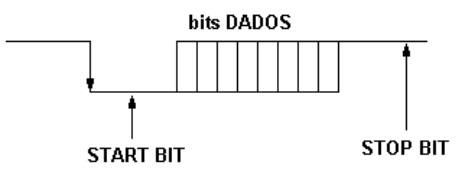
\includegraphics[scale=1]
            {imagens/rs232.jpg}
            \caption{Protocolo RS-232}
            \label{rs232}
        \end{figure}
    
        
    
    \subsection{Parte 2 - Comunicação Serial e interrupções}
        Nesta parte os códigos da Parte 1 foram praticamente reutilizados, porém agora com o uso de interrupções para indicar o envio e a chegada de mensagens pela porta serial. O bit ES liga/desliga a interrupção serial, dependendo de seu estado lógico, e os bits RI e TI são flags que indicam que a mensagem foi enviada e recebida, respectivamente.\\
        

            
    \subsection{Parte 3 - Display de 7 Segmentos}
        Foi proposto a escrita de um número de 4 dígitos nos displays  de 7 segmentos. Como a saída de cada pino do microcontrolador entra na base de um transistor que tem seu coletor no VCC e seu emissor no anodo de cada led, é necessário estar em tensão alta para que o led acenda. O catodo de cada led está ligado em outro pino, que deverá estar em tensão baixa, portanto, para que o led acenda.\\
        
        A figura \ref{display} mostra como os pinos do display estão conectados com o microcontrolador. CN1 e CN2 são os cabos que serão ligados à algum \emph{port} do microcontrolador.\\
        
        A figura \ref{display_bits} mostra o nome de cada led, bem como a qual bit do port ele está conectado.\\
        
        \begin{figure}[H]
            \centering
            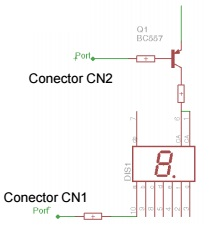
\includegraphics[scale=1]
            {imagens/display_cn.jpg}
            \caption{Conexão dos pinos do display}
            \label{display}
        \end{figure}
            
        \begin{figure}[H]
            \centering
            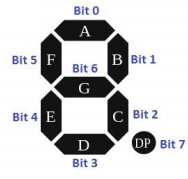
\includegraphics[scale=1]
            {imagens/display_bits.jpg}
            \caption{Numeração dos led's do display}
            \label{display_bits}
        \end{figure}
            
        
    \subsection{Parte 4 - Botão e Chave}
        Cada \emph{port} do microcontrolador contém um latch para cada pino. Em cada pino pode-se ler e escrever valores, porém o valor lido depende do que está pendurado no nó do pino. Pode-se então ler um valor de um botão, fazendo-se a devida montagem. é importante, porém, contornar o problema do ruido do botão, o que normalmente se faz com uma rotina de espera de tempo. \\
        
        A proposta foi implementar um código que leia quais botões estão pressionados, e acende os led's correspondentes da placa. A montagem do botão está representada na figura \ref{button_cn}.\\
        
        \begin{figure}[H]
            \centering
            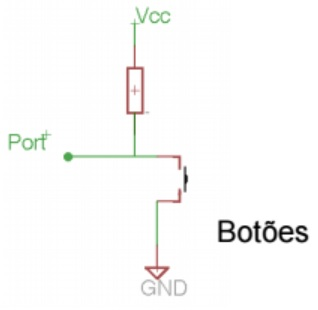
\includegraphics[scale=1]
            {imagens/button_cn.jpg}
            \caption{Conexão do botão ao \emph{port} do microcontrolador}
            \label{button_cn}
        \end{figure}
        
    \subsection{Parte 5 - Display LCD}
        
        O display LCD é um dispositivo um pouco mais complexo que os demais utilizados até agora. Por conter um controladorr dentro de si, ele precisa receber configurações através dos pinos R/W e R/S. As rotinas INIT, POS e WRITE, presentes em quase todos os códigos como será visto, fazem essa configuração para que a escrita seja feita da forma correta.\\
        
        Para se enviar cada comando, é necessário que o LCD receba uma descida de sinal no pino ENAB. A figura \ref{lcd} mostra todos os comandos que se pode dar ao LCD para escrever dados, mover o cursor, ligar o display, entre outros.\\

        \begin{figure}[H]
            \centering
            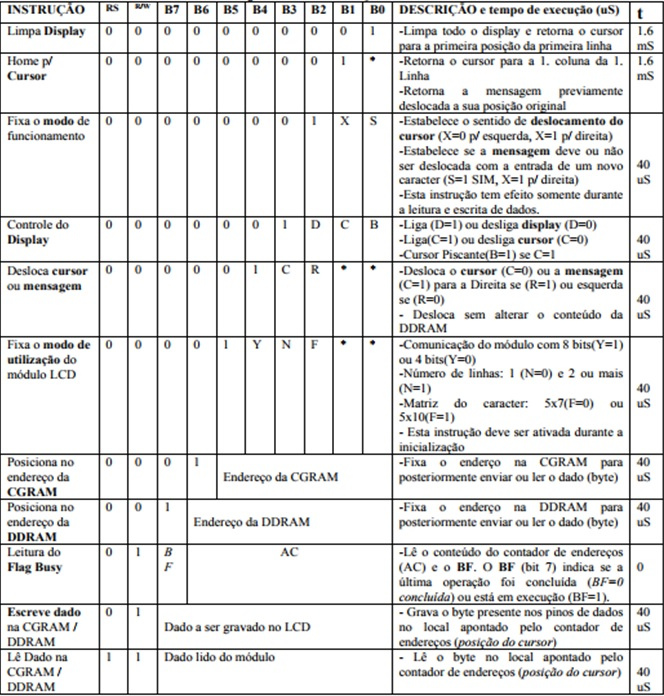
\includegraphics[scale=1]
            {imagens/lcd.jpg}
            \caption{Lista de comandos do LCD}
            \label{lcd}
        \end{figure}

\section{Resultados}

    \subsection{Parte 1}
    \subsection{Parte 2}
    \subsection{Parte 3}
    \subsection{Parte 4}
    \subsection{Parte 5}

\section{Conclusão}

\section{Bibliografia}

\end{document}
